\section{Durchführung}
\label{sec:Durchführung}

\subsection{Versuchsaufbau}
Der Aufbau des Versuchs ist in \autoref{fig:abb2} dargestellt. Das wichtigste Bauteil sind die Kondensatorplatten, die einen Abstand von $d = (7,6250 \pm 0,005) \unit{\milli\meter}$ haben.
In der Mitte oberen Platte befindet sich ein Loch. Durch dieses Loch werden die Öltröpfchen mit einem Zerstäuber eingesprüht.
Die Dichte des verwendeten Öls beträgt $\rho_{öl} = 886 \unit{kilo\gram} \mathbin{/} m^3$. Der Raum zwischen den Platten kann mit einer Halogenlampe $8$ beleuchtet werden, um die Öltröpfchen mit dem Mikroskop $5$ besser beobachten zu können.
$4$ ist der Schalter für ein Thorium-232 Prä­pa­rat. Die meisten Öltröpfchen sollten ionisiert in die Kammer gelangen, jedoch kann die Ladung der einzelnen Tröpfchen mit dem $\alpha$ nachjustiert werden. Dieser Schalter hat drei Positionen.



\begin{figure}[H]
    \centering
    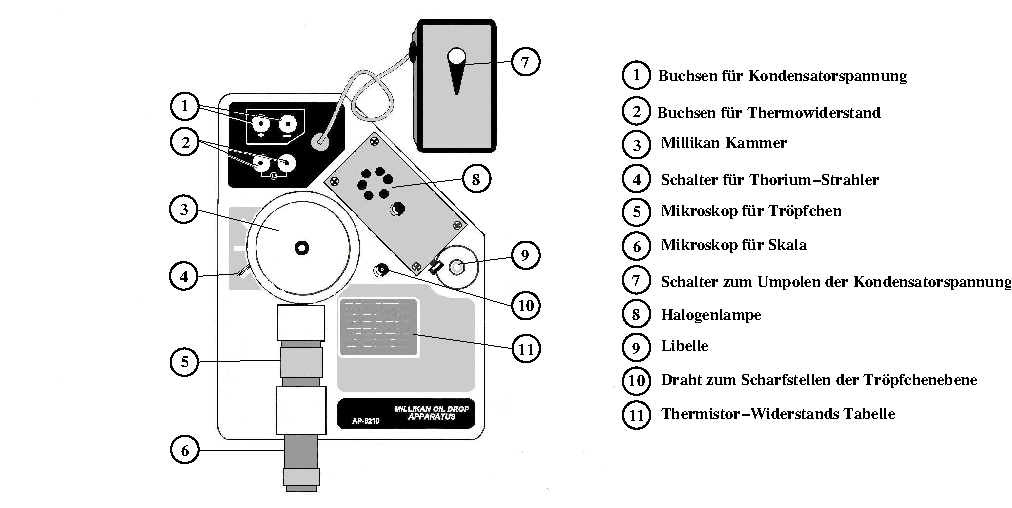
\includegraphics{figures/Abb2.pdf}
    \caption{Aufbau des Millikan-Öltröpfchenversuchs \cite{ap12}.}
    \label{fig:abb2}
\end{figure}